
% Default to the notebook output style

    


% Inherit from the specified cell style.




    
\documentclass[12pt]{article}

    
    
    \usepackage[T1]{fontenc}
    % Nicer default font (+ math font) than Computer Modern for most use cases
    \usepackage{mathpazo}

    % Basic figure setup, for now with no caption control since it's done
    % automatically by Pandoc (which extracts ![](path) syntax from Markdown).
    \usepackage{graphicx}
    % We will generate all images so they have a width \maxwidth. This means
    % that they will get their normal width if they fit onto the page, but
    % are scaled down if they would overflow the margins.
    \makeatletter
    \def\maxwidth{\ifdim\Gin@nat@width>\linewidth\linewidth
    \else\Gin@nat@width\fi}
    \makeatother
    \let\Oldincludegraphics\includegraphics
    % Set max figure width to be 80% of text width, for now hardcoded.
    \renewcommand{\includegraphics}[1]{\Oldincludegraphics[width=.8\maxwidth]{#1}}
    % Ensure that by default, figures have no caption (until we provide a
    % proper Figure object with a Caption API and a way to capture that
    % in the conversion process - todo).
    \usepackage{caption}
    \DeclareCaptionLabelFormat{nolabel}{}
    \captionsetup{labelformat=nolabel}

    \usepackage{adjustbox} % Used to constrain images to a maximum size 
    \usepackage{xcolor} % Allow colors to be defined
    \usepackage{enumerate} % Needed for markdown enumerations to work
    \usepackage{geometry} % Used to adjust the document margins
    \usepackage{amsmath} % Equations
    \usepackage{amssymb} % Equations
    \usepackage{textcomp} % defines textquotesingle
    % Hack from http://tex.stackexchange.com/a/47451/13684:
    \AtBeginDocument{%
        \def\PYZsq{\textquotesingle}% Upright quotes in Pygmentized code
    }
    \usepackage{upquote} % Upright quotes for verbatim code
    \usepackage{eurosym} % defines \euro
    \usepackage[mathletters]{ucs} % Extended unicode (utf-8) support
    \usepackage[utf8x]{inputenc} % Allow utf-8 characters in the tex document
    \usepackage{fancyvrb} % verbatim replacement that allows latex
    \usepackage{grffile} % extends the file name processing of package graphics 
                         % to support a larger range 
    % The hyperref package gives us a pdf with properly built
    % internal navigation ('pdf bookmarks' for the table of contents,
    % internal cross-reference links, web links for URLs, etc.)
    \usepackage{hyperref}
    \usepackage{longtable} % longtable support required by pandoc >1.10
    \usepackage{booktabs}  % table support for pandoc > 1.12.2
    \usepackage[inline]{enumitem} % IRkernel/repr support (it uses the enumerate* environment)
    \usepackage[normalem]{ulem} % ulem is needed to support strikethroughs (\sout)
                                % normalem makes italics be italics, not underlines
    

    
    
    % Colors for the hyperref package
    \definecolor{urlcolor}{rgb}{0,.145,.698}
    \definecolor{linkcolor}{rgb}{.71,0.21,0.01}
    \definecolor{citecolor}{rgb}{.12,.54,.11}

    % ANSI colors
    \definecolor{ansi-black}{HTML}{3E424D}
    \definecolor{ansi-black-intense}{HTML}{282C36}
    \definecolor{ansi-red}{HTML}{E75C58}
    \definecolor{ansi-red-intense}{HTML}{B22B31}
    \definecolor{ansi-green}{HTML}{00A250}
    \definecolor{ansi-green-intense}{HTML}{007427}
    \definecolor{ansi-yellow}{HTML}{DDB62B}
    \definecolor{ansi-yellow-intense}{HTML}{B27D12}
    \definecolor{ansi-blue}{HTML}{208FFB}
    \definecolor{ansi-blue-intense}{HTML}{0065CA}
    \definecolor{ansi-magenta}{HTML}{D160C4}
    \definecolor{ansi-magenta-intense}{HTML}{A03196}
    \definecolor{ansi-cyan}{HTML}{60C6C8}
    \definecolor{ansi-cyan-intense}{HTML}{258F8F}
    \definecolor{ansi-white}{HTML}{C5C1B4}
    \definecolor{ansi-white-intense}{HTML}{A1A6B2}

    % commands and environments needed by pandoc snippets
    % extracted from the output of `pandoc -s`
    \providecommand{\tightlist}{%
      \setlength{\itemsep}{0pt}\setlength{\parskip}{0pt}}
    \DefineVerbatimEnvironment{Highlighting}{Verbatim}{commandchars=\\\{\}}
    % Add ',fontsize=\small' for more characters per line
    \newenvironment{Shaded}{}{}
    \newcommand{\KeywordTok}[1]{\textcolor[rgb]{0.00,0.44,0.13}{\textbf{{#1}}}}
    \newcommand{\DataTypeTok}[1]{\textcolor[rgb]{0.56,0.13,0.00}{{#1}}}
    \newcommand{\DecValTok}[1]{\textcolor[rgb]{0.25,0.63,0.44}{{#1}}}
    \newcommand{\BaseNTok}[1]{\textcolor[rgb]{0.25,0.63,0.44}{{#1}}}
    \newcommand{\FloatTok}[1]{\textcolor[rgb]{0.25,0.63,0.44}{{#1}}}
    \newcommand{\CharTok}[1]{\textcolor[rgb]{0.25,0.44,0.63}{{#1}}}
    \newcommand{\StringTok}[1]{\textcolor[rgb]{0.25,0.44,0.63}{{#1}}}
    \newcommand{\CommentTok}[1]{\textcolor[rgb]{0.38,0.63,0.69}{\textit{{#1}}}}
    \newcommand{\OtherTok}[1]{\textcolor[rgb]{0.00,0.44,0.13}{{#1}}}
    \newcommand{\AlertTok}[1]{\textcolor[rgb]{1.00,0.00,0.00}{\textbf{{#1}}}}
    \newcommand{\FunctionTok}[1]{\textcolor[rgb]{0.02,0.16,0.49}{{#1}}}
    \newcommand{\RegionMarkerTok}[1]{{#1}}
    \newcommand{\ErrorTok}[1]{\textcolor[rgb]{1.00,0.00,0.00}{\textbf{{#1}}}}
    \newcommand{\NormalTok}[1]{{#1}}
    
    % Additional commands for more recent versions of Pandoc
    \newcommand{\ConstantTok}[1]{\textcolor[rgb]{0.53,0.00,0.00}{{#1}}}
    \newcommand{\SpecialCharTok}[1]{\textcolor[rgb]{0.25,0.44,0.63}{{#1}}}
    \newcommand{\VerbatimStringTok}[1]{\textcolor[rgb]{0.25,0.44,0.63}{{#1}}}
    \newcommand{\SpecialStringTok}[1]{\textcolor[rgb]{0.73,0.40,0.53}{{#1}}}
    \newcommand{\ImportTok}[1]{{#1}}
    \newcommand{\DocumentationTok}[1]{\textcolor[rgb]{0.73,0.13,0.13}{\textit{{#1}}}}
    \newcommand{\AnnotationTok}[1]{\textcolor[rgb]{0.38,0.63,0.69}{\textbf{\textit{{#1}}}}}
    \newcommand{\CommentVarTok}[1]{\textcolor[rgb]{0.38,0.63,0.69}{\textbf{\textit{{#1}}}}}
    \newcommand{\VariableTok}[1]{\textcolor[rgb]{0.10,0.09,0.49}{{#1}}}
    \newcommand{\ControlFlowTok}[1]{\textcolor[rgb]{0.00,0.44,0.13}{\textbf{{#1}}}}
    \newcommand{\OperatorTok}[1]{\textcolor[rgb]{0.40,0.40,0.40}{{#1}}}
    \newcommand{\BuiltInTok}[1]{{#1}}
    \newcommand{\ExtensionTok}[1]{{#1}}
    \newcommand{\PreprocessorTok}[1]{\textcolor[rgb]{0.74,0.48,0.00}{{#1}}}
    \newcommand{\AttributeTok}[1]{\textcolor[rgb]{0.49,0.56,0.16}{{#1}}}
    \newcommand{\InformationTok}[1]{\textcolor[rgb]{0.38,0.63,0.69}{\textbf{\textit{{#1}}}}}
    \newcommand{\WarningTok}[1]{\textcolor[rgb]{0.38,0.63,0.69}{\textbf{\textit{{#1}}}}}
    
    
    % Define a nice break command that doesn't care if a line doesn't already
    % exist.
    \def\br{\hspace*{\fill} \\* }
    % Math Jax compatability definitions
    \def\gt{>}
    \def\lt{<}
    % Document parameters
    \title{P1 ICA Implementation}
    \author{William Koehrsen wjk68}
    \date{April 25, 2018}
    
   
    % Pygments definitions
    
\makeatletter
\def\PY@reset{\let\PY@it=\relax \let\PY@bf=\relax%
    \let\PY@ul=\relax \let\PY@tc=\relax%
    \let\PY@bc=\relax \let\PY@ff=\relax}
\def\PY@tok#1{\csname PY@tok@#1\endcsname}
\def\PY@toks#1+{\ifx\relax#1\empty\else%
    \PY@tok{#1}\expandafter\PY@toks\fi}
\def\PY@do#1{\PY@bc{\PY@tc{\PY@ul{%
    \PY@it{\PY@bf{\PY@ff{#1}}}}}}}
\def\PY#1#2{\PY@reset\PY@toks#1+\relax+\PY@do{#2}}

\expandafter\def\csname PY@tok@w\endcsname{\def\PY@tc##1{\textcolor[rgb]{0.73,0.73,0.73}{##1}}}
\expandafter\def\csname PY@tok@c\endcsname{\let\PY@it=\textit\def\PY@tc##1{\textcolor[rgb]{0.25,0.50,0.50}{##1}}}
\expandafter\def\csname PY@tok@cp\endcsname{\def\PY@tc##1{\textcolor[rgb]{0.74,0.48,0.00}{##1}}}
\expandafter\def\csname PY@tok@k\endcsname{\let\PY@bf=\textbf\def\PY@tc##1{\textcolor[rgb]{0.00,0.50,0.00}{##1}}}
\expandafter\def\csname PY@tok@kp\endcsname{\def\PY@tc##1{\textcolor[rgb]{0.00,0.50,0.00}{##1}}}
\expandafter\def\csname PY@tok@kt\endcsname{\def\PY@tc##1{\textcolor[rgb]{0.69,0.00,0.25}{##1}}}
\expandafter\def\csname PY@tok@o\endcsname{\def\PY@tc##1{\textcolor[rgb]{0.40,0.40,0.40}{##1}}}
\expandafter\def\csname PY@tok@ow\endcsname{\let\PY@bf=\textbf\def\PY@tc##1{\textcolor[rgb]{0.67,0.13,1.00}{##1}}}
\expandafter\def\csname PY@tok@nb\endcsname{\def\PY@tc##1{\textcolor[rgb]{0.00,0.50,0.00}{##1}}}
\expandafter\def\csname PY@tok@nf\endcsname{\def\PY@tc##1{\textcolor[rgb]{0.00,0.00,1.00}{##1}}}
\expandafter\def\csname PY@tok@nc\endcsname{\let\PY@bf=\textbf\def\PY@tc##1{\textcolor[rgb]{0.00,0.00,1.00}{##1}}}
\expandafter\def\csname PY@tok@nn\endcsname{\let\PY@bf=\textbf\def\PY@tc##1{\textcolor[rgb]{0.00,0.00,1.00}{##1}}}
\expandafter\def\csname PY@tok@ne\endcsname{\let\PY@bf=\textbf\def\PY@tc##1{\textcolor[rgb]{0.82,0.25,0.23}{##1}}}
\expandafter\def\csname PY@tok@nv\endcsname{\def\PY@tc##1{\textcolor[rgb]{0.10,0.09,0.49}{##1}}}
\expandafter\def\csname PY@tok@no\endcsname{\def\PY@tc##1{\textcolor[rgb]{0.53,0.00,0.00}{##1}}}
\expandafter\def\csname PY@tok@nl\endcsname{\def\PY@tc##1{\textcolor[rgb]{0.63,0.63,0.00}{##1}}}
\expandafter\def\csname PY@tok@ni\endcsname{\let\PY@bf=\textbf\def\PY@tc##1{\textcolor[rgb]{0.60,0.60,0.60}{##1}}}
\expandafter\def\csname PY@tok@na\endcsname{\def\PY@tc##1{\textcolor[rgb]{0.49,0.56,0.16}{##1}}}
\expandafter\def\csname PY@tok@nt\endcsname{\let\PY@bf=\textbf\def\PY@tc##1{\textcolor[rgb]{0.00,0.50,0.00}{##1}}}
\expandafter\def\csname PY@tok@nd\endcsname{\def\PY@tc##1{\textcolor[rgb]{0.67,0.13,1.00}{##1}}}
\expandafter\def\csname PY@tok@s\endcsname{\def\PY@tc##1{\textcolor[rgb]{0.73,0.13,0.13}{##1}}}
\expandafter\def\csname PY@tok@sd\endcsname{\let\PY@it=\textit\def\PY@tc##1{\textcolor[rgb]{0.73,0.13,0.13}{##1}}}
\expandafter\def\csname PY@tok@si\endcsname{\let\PY@bf=\textbf\def\PY@tc##1{\textcolor[rgb]{0.73,0.40,0.53}{##1}}}
\expandafter\def\csname PY@tok@se\endcsname{\let\PY@bf=\textbf\def\PY@tc##1{\textcolor[rgb]{0.73,0.40,0.13}{##1}}}
\expandafter\def\csname PY@tok@sr\endcsname{\def\PY@tc##1{\textcolor[rgb]{0.73,0.40,0.53}{##1}}}
\expandafter\def\csname PY@tok@ss\endcsname{\def\PY@tc##1{\textcolor[rgb]{0.10,0.09,0.49}{##1}}}
\expandafter\def\csname PY@tok@sx\endcsname{\def\PY@tc##1{\textcolor[rgb]{0.00,0.50,0.00}{##1}}}
\expandafter\def\csname PY@tok@m\endcsname{\def\PY@tc##1{\textcolor[rgb]{0.40,0.40,0.40}{##1}}}
\expandafter\def\csname PY@tok@gh\endcsname{\let\PY@bf=\textbf\def\PY@tc##1{\textcolor[rgb]{0.00,0.00,0.50}{##1}}}
\expandafter\def\csname PY@tok@gu\endcsname{\let\PY@bf=\textbf\def\PY@tc##1{\textcolor[rgb]{0.50,0.00,0.50}{##1}}}
\expandafter\def\csname PY@tok@gd\endcsname{\def\PY@tc##1{\textcolor[rgb]{0.63,0.00,0.00}{##1}}}
\expandafter\def\csname PY@tok@gi\endcsname{\def\PY@tc##1{\textcolor[rgb]{0.00,0.63,0.00}{##1}}}
\expandafter\def\csname PY@tok@gr\endcsname{\def\PY@tc##1{\textcolor[rgb]{1.00,0.00,0.00}{##1}}}
\expandafter\def\csname PY@tok@ge\endcsname{\let\PY@it=\textit}
\expandafter\def\csname PY@tok@gs\endcsname{\let\PY@bf=\textbf}
\expandafter\def\csname PY@tok@gp\endcsname{\let\PY@bf=\textbf\def\PY@tc##1{\textcolor[rgb]{0.00,0.00,0.50}{##1}}}
\expandafter\def\csname PY@tok@go\endcsname{\def\PY@tc##1{\textcolor[rgb]{0.53,0.53,0.53}{##1}}}
\expandafter\def\csname PY@tok@gt\endcsname{\def\PY@tc##1{\textcolor[rgb]{0.00,0.27,0.87}{##1}}}
\expandafter\def\csname PY@tok@err\endcsname{\def\PY@bc##1{\setlength{\fboxsep}{0pt}\fcolorbox[rgb]{1.00,0.00,0.00}{1,1,1}{\strut ##1}}}
\expandafter\def\csname PY@tok@kc\endcsname{\let\PY@bf=\textbf\def\PY@tc##1{\textcolor[rgb]{0.00,0.50,0.00}{##1}}}
\expandafter\def\csname PY@tok@kd\endcsname{\let\PY@bf=\textbf\def\PY@tc##1{\textcolor[rgb]{0.00,0.50,0.00}{##1}}}
\expandafter\def\csname PY@tok@kn\endcsname{\let\PY@bf=\textbf\def\PY@tc##1{\textcolor[rgb]{0.00,0.50,0.00}{##1}}}
\expandafter\def\csname PY@tok@kr\endcsname{\let\PY@bf=\textbf\def\PY@tc##1{\textcolor[rgb]{0.00,0.50,0.00}{##1}}}
\expandafter\def\csname PY@tok@bp\endcsname{\def\PY@tc##1{\textcolor[rgb]{0.00,0.50,0.00}{##1}}}
\expandafter\def\csname PY@tok@fm\endcsname{\def\PY@tc##1{\textcolor[rgb]{0.00,0.00,1.00}{##1}}}
\expandafter\def\csname PY@tok@vc\endcsname{\def\PY@tc##1{\textcolor[rgb]{0.10,0.09,0.49}{##1}}}
\expandafter\def\csname PY@tok@vg\endcsname{\def\PY@tc##1{\textcolor[rgb]{0.10,0.09,0.49}{##1}}}
\expandafter\def\csname PY@tok@vi\endcsname{\def\PY@tc##1{\textcolor[rgb]{0.10,0.09,0.49}{##1}}}
\expandafter\def\csname PY@tok@vm\endcsname{\def\PY@tc##1{\textcolor[rgb]{0.10,0.09,0.49}{##1}}}
\expandafter\def\csname PY@tok@sa\endcsname{\def\PY@tc##1{\textcolor[rgb]{0.73,0.13,0.13}{##1}}}
\expandafter\def\csname PY@tok@sb\endcsname{\def\PY@tc##1{\textcolor[rgb]{0.73,0.13,0.13}{##1}}}
\expandafter\def\csname PY@tok@sc\endcsname{\def\PY@tc##1{\textcolor[rgb]{0.73,0.13,0.13}{##1}}}
\expandafter\def\csname PY@tok@dl\endcsname{\def\PY@tc##1{\textcolor[rgb]{0.73,0.13,0.13}{##1}}}
\expandafter\def\csname PY@tok@s2\endcsname{\def\PY@tc##1{\textcolor[rgb]{0.73,0.13,0.13}{##1}}}
\expandafter\def\csname PY@tok@sh\endcsname{\def\PY@tc##1{\textcolor[rgb]{0.73,0.13,0.13}{##1}}}
\expandafter\def\csname PY@tok@s1\endcsname{\def\PY@tc##1{\textcolor[rgb]{0.73,0.13,0.13}{##1}}}
\expandafter\def\csname PY@tok@mb\endcsname{\def\PY@tc##1{\textcolor[rgb]{0.40,0.40,0.40}{##1}}}
\expandafter\def\csname PY@tok@mf\endcsname{\def\PY@tc##1{\textcolor[rgb]{0.40,0.40,0.40}{##1}}}
\expandafter\def\csname PY@tok@mh\endcsname{\def\PY@tc##1{\textcolor[rgb]{0.40,0.40,0.40}{##1}}}
\expandafter\def\csname PY@tok@mi\endcsname{\def\PY@tc##1{\textcolor[rgb]{0.40,0.40,0.40}{##1}}}
\expandafter\def\csname PY@tok@il\endcsname{\def\PY@tc##1{\textcolor[rgb]{0.40,0.40,0.40}{##1}}}
\expandafter\def\csname PY@tok@mo\endcsname{\def\PY@tc##1{\textcolor[rgb]{0.40,0.40,0.40}{##1}}}
\expandafter\def\csname PY@tok@ch\endcsname{\let\PY@it=\textit\def\PY@tc##1{\textcolor[rgb]{0.25,0.50,0.50}{##1}}}
\expandafter\def\csname PY@tok@cm\endcsname{\let\PY@it=\textit\def\PY@tc##1{\textcolor[rgb]{0.25,0.50,0.50}{##1}}}
\expandafter\def\csname PY@tok@cpf\endcsname{\let\PY@it=\textit\def\PY@tc##1{\textcolor[rgb]{0.25,0.50,0.50}{##1}}}
\expandafter\def\csname PY@tok@c1\endcsname{\let\PY@it=\textit\def\PY@tc##1{\textcolor[rgb]{0.25,0.50,0.50}{##1}}}
\expandafter\def\csname PY@tok@cs\endcsname{\let\PY@it=\textit\def\PY@tc##1{\textcolor[rgb]{0.25,0.50,0.50}{##1}}}

\def\PYZbs{\char`\\}
\def\PYZus{\char`\_}
\def\PYZob{\char`\{}
\def\PYZcb{\char`\}}
\def\PYZca{\char`\^}
\def\PYZam{\char`\&}
\def\PYZlt{\char`\<}
\def\PYZgt{\char`\>}
\def\PYZsh{\char`\#}
\def\PYZpc{\char`\%}
\def\PYZdl{\char`\$}
\def\PYZhy{\char`\-}
\def\PYZsq{\char`\'}
\def\PYZdq{\char`\"}
\def\PYZti{\char`\~}
% for compatibility with earlier versions
\def\PYZat{@}
\def\PYZlb{[}
\def\PYZrb{]}
\makeatother


    % Exact colors from NB
    \definecolor{incolor}{rgb}{0.0, 0.0, 0.5}
    \definecolor{outcolor}{rgb}{0.545, 0.0, 0.0}



    
    % Prevent overflowing lines due to hard-to-break entities
    \sloppy 
    % Setup hyperref package
    \hypersetup{
      breaklinks=true,  % so long urls are correctly broken across lines
      colorlinks=true,
      urlcolor=urlcolor,
      linkcolor=blue,
      citecolor=citecolor,
      }
    % Slightly bigger margins than the latex defaults
    
    \geometry{verbose,tmargin=1in,bmargin=1in,lmargin=1in,rmargin=1in}

    \begin{document}
    
    
    \maketitle
    \tableofcontents
    

    
    \hypertarget{introduction}{%
\section{Introduction: FastICA Implementation}\label{introduction}}

In this notebook, we look at implementing independent component analysis
(ICA). This method can be used for blind source separation, or in other
words, to determine the independent individual signals comprising a
single mixed signal. Applications of ICA include separating out the
individual parts of audio signals or dimensionality reduction for
classification/regression machine learning models. For example, if there
are 3 instruments playing at the same time, ICA can be used to separate
out the individual instruments from the composite signal. The components
returned by ICA are maximally independent, which means that information
on one component does not give information on the other components. ICA
operates under the assumption that the components are independent and
non-Gaussian.

    \begin{Verbatim}[commandchars=\\\{\}]
{\color{incolor}In [{\color{incolor}1}]:} \PY{c+c1}{\PYZsh{} Pandas and numpy for data manipulation}
        \PY{k+kn}{import} \PY{n+nn}{pandas} \PY{k}{as} \PY{n+nn}{pd}
        \PY{k+kn}{import} \PY{n+nn}{numpy} \PY{k}{as} \PY{n+nn}{np}
\end{Verbatim}


    \begin{Verbatim}[commandchars=\\\{\}]
{\color{incolor}In [{\color{incolor}2}]:} \PY{c+c1}{\PYZsh{} Utilities for linear algebra }
        \PY{k+kn}{from} \PY{n+nn}{scipy} \PY{k}{import} \PY{n}{linalg}
        
        \PY{c+c1}{\PYZsh{} Convergence check}
        \PY{k+kn}{import} \PY{n+nn}{warnings}
\end{Verbatim}


    \hypertarget{implementation-of-fastica}{%
\section{Implementation of FastICA}\label{implementation-of-fastica}}

The particular implementation of Independent Component Analysis we will
use here is known as fast ica. Reference for this method can be found in
\href{https://www.cs.helsinki.fi/u/ahyvarin/papers/NN00new.pdf}{the
paper} ``Independent Component Analysis: Algorithms and Applications''
by Aapo Hyvärinen and Erkki Oja.

Additional information on ICA used in the report can be found in
\href{https://www.cs.helsinki.fi/u/ahyvarin/papers/bookfinal_ICA.pdf}{this
book}. In particular, the algorithm is developed using information
presented in Chapter 8 (pages 165-199).

A third source consulted for this method was
\href{http://www.ccs.neu.edu/home/jaa/CS6800.11F/Topics/Papers/Hyvarinen97.pdf}{the
paper} ``Independent Component Analysis by Minimization of Mutual
Information'' by Aapo Hyvärinen.

ICA assumes the data matrix, X, to be a linear combination of
non-Gaussian (independent) components. In other words,
\(X = \text{mixing} * \text{source}\) where mixing and source are both
matrices (this equation is generally written as \(X = AS\)). The columns
of the source matrix contain the independent components, and A is the
linear mixing matrix. The objective of ICA is to un-mix the data by
finding the un-mixing matrix (W). The source matrix, S, can then be
found from \(S = W K X\) where K is a pre-whitening matrix that projects
the data matrix onto the principal components.

When running ICA, we need to specify a number of components,
\texttt{n\_components}. The shape of the matrices are:

\begin{itemize}
\tightlist
\item
  X, data matrix: {[}\texttt{n\_samples,\ n\_features}{]}
\item
  S, source matrix: {[}\texttt{n\_samples,\ n\_components}{]}
\item
  W, un-mixing matrix: {[}\texttt{n\_components,\ n\_features}{]}
\item
  K, whitening matrix: {[}\texttt{n\_components,\ n\_features}{]}
\end{itemize}

Once the S, W, and K matrices have been found, the mixing matrix can be
calculated from \(A = WK^-1\) where the shape is
{[}\texttt{n\_features,\ n\_components}{]}.

    \hypertarget{utility-function-negentropy}{%
\subsection{Utility Function:
Negentropy}\label{utility-function-negentropy}}

The cost function used in ICA is the negative entropy, negentropy.
Negative entropy is a measure of non-Gaussianity that is based on the
information-theroy quantity of entropy. The more unpredictable a
variable, the greater its entropy. A Gaussian random variable has
maximum entropy. Rather than using entropy, we will use a measure called
negentropy, which is always non-negative and zero if and only if the
variable has a Gaussian distribution. Therefore, if the utility function
is Negentropy, the goal is to maximize this quantity. The definition of
Negentropy is:

\[J(y) = H(y_{gauss}) - H(y)\]

where \(y_{gauss}\) is a random Gaussian varialbe with the same
covariance matrix as \(y\).

This follows from the definition of Entropy for a continuous variable:

\[H(y) = -\int{f(y)\log{f(y)}d(y)}\]

Negentropy is extremely computationally expensive to calculate because
it requires estimation of the probability density function (pdf).
Therefore approximations of Negentropy are used in practice. In this
notebook we will be using the following approximation.

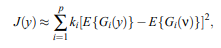
\includegraphics{../images/negentropy_approximation.png}

Where \(v\) is a Guassian variable of zero mean and unit variance,
\(k_i\) are positive constants, the variable \(y\) has zero mean and
unit variance, and \(G_i\) are nonquadratic functions. We will use a
single non-quadratic function. Good choices for \(G\) are functions that
do not grow too fast.

The following is the log cosh function that we will be using for the
non-quadratic function:

\[G_1(u) = \frac{1}{a_1}\log{\cosh{a_1u}}\]

Here \(1 \le{a_1}\le{2}\) and the overall method gives a good
approximation of Negentropy.

We can use the identity

\[\frac{d}{dx}(\log{\cosh{x}}) = \tanh{x}\]

    \begin{Verbatim}[commandchars=\\\{\}]
{\color{incolor}In [{\color{incolor}3}]:} \PY{c+c1}{\PYZsh{} Calculate g and g\PYZus{} for a function}
        \PY{c+c1}{\PYZsh{} Standard non\PYZus{}linear function}
        \PY{k}{def} \PY{n+nf}{logcosh}\PY{p}{(}\PY{n}{x}\PY{p}{,} \PY{n}{alpha} \PY{o}{=} \PY{l+m+mf}{1.0}\PY{p}{)}\PY{p}{:}
        
            \PY{n}{x} \PY{o}{*}\PY{o}{=} \PY{n}{alpha}
            
            \PY{c+c1}{\PYZsh{} Apply tanh inplace}
            \PY{c+c1}{\PYZsh{} Using the identity that the deri}
            \PY{n}{gx} \PY{o}{=} \PY{n}{np}\PY{o}{.}\PY{n}{tanh}\PY{p}{(}\PY{n}{x}\PY{p}{,} \PY{n}{x}\PY{p}{)}
            \PY{n}{g\PYZus{}x} \PY{o}{=} \PY{n}{np}\PY{o}{.}\PY{n}{empty}\PY{p}{(}\PY{n}{x}\PY{o}{.}\PY{n}{shape}\PY{p}{[}\PY{l+m+mi}{0}\PY{p}{]}\PY{p}{)}
            
            \PY{k}{for} \PY{n}{i}\PY{p}{,} \PY{n}{gx\PYZus{}i} \PY{o+ow}{in} \PY{n+nb}{enumerate}\PY{p}{(}\PY{n}{gx}\PY{p}{)}\PY{p}{:}
                \PY{n}{g\PYZus{}x}\PY{p}{[}\PY{n}{i}\PY{p}{]} \PY{o}{=} \PY{p}{(}\PY{n}{alpha} \PY{o}{*} \PY{p}{(}\PY{l+m+mi}{1} \PY{o}{\PYZhy{}} \PY{n}{gx\PYZus{}i} \PY{o}{*}\PY{o}{*} \PY{l+m+mi}{2}\PY{p}{)}\PY{p}{)}\PY{o}{.}\PY{n}{mean}\PY{p}{(}\PY{p}{)}
                
            \PY{k}{return} \PY{n}{gx}\PY{p}{,} \PY{n}{g\PYZus{}x}
\end{Verbatim}


    \hypertarget{preprocessing}{%
\section{Preprocessing}\label{preprocessing}}

\hypertarget{centering}{%
\subsection{Centering}\label{centering}}

This simply entails subtracting the mean from each feature of a sample.
The resulting variable is a zero-mean variable. The mean can be added
back into the centered sources after the mixing matrix has been
estimated with the centered data. Also, to re-construct the original
signal, we need to add the mean back into the product of the mixing and
source matrices.

    \hypertarget{whitening-components}{%
\subsection{Whitening Components}\label{whitening-components}}

The observed variables must be whitened after they are centered.
Whitening results in a new vector that has uncorrelated coponents with
variances equal to unity. The result is that the covariance matix of the
vector quals the identity matrix.

Here we will use the eigenvalue decomposition of the convariance matrix
to whiten the components. The whitening process reudcues the number of
parameters that need to be estaimed because the new mixing matrix is
orthogonal. This reduces the degrees of freedom and reduces the
complexity of the independent component analysis problem.

    \begin{Verbatim}[commandchars=\\\{\}]
{\color{incolor}In [{\color{incolor}4}]:} \PY{c+c1}{\PYZsh{} Center and Whiten components}
        \PY{k}{def} \PY{n+nf}{whiten\PYZus{}components}\PY{p}{(}\PY{n}{X}\PY{p}{,} \PY{n}{n\PYZus{}components}\PY{p}{)}\PY{p}{:}
            
            \PY{n}{n}\PY{p}{,} \PY{n}{p} \PY{o}{=} \PY{n}{X}\PY{o}{.}\PY{n}{shape}
        
            \PY{n}{X\PYZus{}mean} \PY{o}{=} \PY{n}{X}\PY{o}{.}\PY{n}{mean}\PY{p}{(}\PY{n}{axis}\PY{o}{=}\PY{o}{\PYZhy{}}\PY{l+m+mi}{1}\PY{p}{)}
            
            \PY{c+c1}{\PYZsh{} Subtract the mean for 0 mean}
            \PY{n}{X} \PY{o}{\PYZhy{}}\PY{o}{=} \PY{n}{X\PYZus{}mean}\PY{p}{[}\PY{p}{:}\PY{p}{,} \PY{n}{np}\PY{o}{.}\PY{n}{newaxis}\PY{p}{]}
            
            \PY{c+c1}{\PYZsh{} Preprocessing by PCA}
            \PY{n}{u}\PY{p}{,} \PY{n}{d}\PY{p}{,} \PY{n}{\PYZus{}} \PY{o}{=} \PY{n}{linalg}\PY{o}{.}\PY{n}{svd}\PY{p}{(}\PY{n}{X}\PY{p}{,} \PY{n}{full\PYZus{}matrices}\PY{o}{=}\PY{k+kc}{False}\PY{p}{)}
            
            \PY{c+c1}{\PYZsh{} Whitening matrix}
            \PY{n}{whitening} \PY{o}{=} \PY{p}{(}\PY{n}{u} \PY{o}{/} \PY{n}{d}\PY{p}{)}\PY{o}{.}\PY{n}{T}\PY{p}{[}\PY{p}{:}\PY{n}{n\PYZus{}components}\PY{p}{]}
            
            \PY{c+c1}{\PYZsh{} Project data onto the principal components using the whitening matrix}
            \PY{n}{X1} \PY{o}{=} \PY{n}{np}\PY{o}{.}\PY{n}{dot}\PY{p}{(}\PY{n}{whitening}\PY{p}{,} \PY{n}{X}\PY{p}{)}
            \PY{n}{X1} \PY{o}{*}\PY{o}{=} \PY{n}{np}\PY{o}{.}\PY{n}{sqrt}\PY{p}{(}\PY{n}{p}\PY{p}{)}
            
            \PY{c+c1}{\PYZsh{} Return whitened components, whitening matrix, and mean of components}
            \PY{k}{return} \PY{n}{X1}\PY{p}{,} \PY{n}{whitening}\PY{p}{,} \PY{n}{X\PYZus{}mean}
\end{Verbatim}


    \hypertarget{symmetric-decorrelation}{%
\subsection{Symmetric Decorrelation}\label{symmetric-decorrelation}}

The outputs must be decorrelated to prevent the vectors from converging
to the same maxima. Decorrelation occurs after every iteration. There
are several methods of decorrelation including deflation, where the
indepedent components are estimated one-by-one, and symmetric where all
the components are estimated at once. This means that no vectors are
privileged over any others.

Symmetric decorrelation is expressed in the following equation:

\[W = (WW^T)^{-\frac{1}{2}}W\]

Where \(W\) is the matrix of the vecots and the inverse square root is
found from the eigenvalue decomposition. There are also iterative
algorithms to determine the symmetric decorrelation.

    \begin{Verbatim}[commandchars=\\\{\}]
{\color{incolor}In [{\color{incolor}5}]:} \PY{c+c1}{\PYZsh{} Symmetric decorrelation of un\PYZus{}mixing matrix}
        \PY{c+c1}{\PYZsh{} Ensures no vectors are privileged over others}
        \PY{k}{def} \PY{n+nf}{symmetric\PYZus{}decorrelation}\PY{p}{(}\PY{n}{un\PYZus{}mixing}\PY{p}{)}\PY{p}{:}
            
            \PY{c+c1}{\PYZsh{} Find eigenvalues and eigenvectors of unmixing matrix}
            \PY{n}{eig\PYZus{}values}\PY{p}{,} \PY{n}{eig\PYZus{}vectors} \PY{o}{=} \PY{n}{linalg}\PY{o}{.}\PY{n}{eigh}\PY{p}{(}\PY{n}{np}\PY{o}{.}\PY{n}{dot}\PY{p}{(}\PY{n}{un\PYZus{}mixing}\PY{p}{,} \PY{n}{un\PYZus{}mixing}\PY{o}{.}\PY{n}{T}\PY{p}{)}\PY{p}{)}
            
            \PY{c+c1}{\PYZsh{} Apply symmetric decorrelation equation}
            \PY{n}{sym\PYZus{}un\PYZus{}mixing} \PY{o}{=} \PY{n}{np}\PY{o}{.}\PY{n}{dot}\PY{p}{(}\PY{n}{np}\PY{o}{.}\PY{n}{dot}\PY{p}{(}\PY{n}{eig\PYZus{}vectors} \PY{o}{*} \PY{p}{(}\PY{l+m+mi}{1} \PY{o}{/} \PY{n}{np}\PY{o}{.}\PY{n}{sqrt}\PY{p}{(}\PY{n}{eig\PYZus{}values}\PY{p}{)}\PY{p}{)}\PY{p}{,} \PY{n}{eig\PYZus{}vectors}\PY{o}{.}\PY{n}{T}\PY{p}{)}\PY{p}{,} \PY{n}{un\PYZus{}mixing}\PY{p}{)}
            
            \PY{k}{return} \PY{n}{sym\PYZus{}un\PYZus{}mixing}
\end{Verbatim}


    \hypertarget{parallel-ica}{%
\section{Parallel ICA}\label{parallel-ica}}

The parallel ica algorithm estimates all of the independent components
at once on each iteration. This requires using the symmetric
decorrelation on each iteration After estimating the components on one
iteration, the Negentropy is calculated. If the Negentropy increase is
below the tolerance, the algorithm stops.

    \begin{Verbatim}[commandchars=\\\{\}]
{\color{incolor}In [{\color{incolor}6}]:} \PY{k}{def} \PY{n+nf}{parallel\PYZus{}ica}\PY{p}{(}\PY{n}{X}\PY{p}{,} \PY{n}{init\PYZus{}un\PYZus{}mixing}\PY{p}{,} \PY{n}{alpha} \PY{o}{=} \PY{l+m+mf}{1.0}\PY{p}{,} \PY{n}{max\PYZus{}iter} \PY{o}{=} \PY{l+m+mi}{1000}\PY{p}{,} \PY{n}{tol} \PY{o}{=} \PY{l+m+mf}{1e\PYZhy{}4}\PY{p}{,} \PY{n}{return\PYZus{}iter} \PY{o}{=} \PY{k+kc}{False}\PY{p}{)}\PY{p}{:}
            
            \PY{c+c1}{\PYZsh{} Symmetric decorrelation of initial un\PYZhy{}mixing components }
            \PY{n}{un\PYZus{}mixing} \PY{o}{=} \PY{n}{symmetric\PYZus{}decorrelation}\PY{p}{(}\PY{n}{init\PYZus{}un\PYZus{}mixing}\PY{p}{)}
            
            
            \PY{n}{p} \PY{o}{=} \PY{n+nb}{float}\PY{p}{(}\PY{n}{X}\PY{o}{.}\PY{n}{shape}\PY{p}{[}\PY{l+m+mi}{1}\PY{p}{]}\PY{p}{)}
            
            \PY{c+c1}{\PYZsh{} Iteratively update the un\PYZhy{}mixing matrix}
            \PY{k}{for} \PY{n}{i} \PY{o+ow}{in} \PY{n+nb}{range}\PY{p}{(}\PY{n}{max\PYZus{}iter}\PY{p}{)}\PY{p}{:}
                
                \PY{c+c1}{\PYZsh{} Function (g) and gradient from the Negentropy approximation}
                \PY{n}{gwtx}\PY{p}{,} \PY{n}{g\PYZus{}wtx} \PY{o}{=} \PY{n}{logcosh}\PY{p}{(}\PY{n}{np}\PY{o}{.}\PY{n}{dot}\PY{p}{(}\PY{n}{un\PYZus{}mixing}\PY{p}{,} \PY{n}{X}\PY{p}{)}\PY{p}{,} \PY{n}{alpha}\PY{p}{)}
                
                \PY{c+c1}{\PYZsh{} Decorrelate the un\PYZhy{}mixing matrix on every loop}
                \PY{n}{new\PYZus{}un\PYZus{}mixing} \PY{o}{=} \PY{n}{symmetric\PYZus{}decorrelation}\PY{p}{(}\PY{n}{np}\PY{o}{.}\PY{n}{dot}\PY{p}{(}\PY{n}{gwtx}\PY{p}{,} \PY{n}{X}\PY{o}{.}\PY{n}{T}\PY{p}{)} \PY{o}{/} \PY{n}{p} \PY{o}{\PYZhy{}} \PY{n}{g\PYZus{}wtx}\PY{p}{[}\PY{p}{:}\PY{p}{,} \PY{n}{np}\PY{o}{.}\PY{n}{newaxis}\PY{p}{]} \PY{o}{*} \PY{n}{un\PYZus{}mixing}\PY{p}{)}
                
                \PY{c+c1}{\PYZsh{} Calculate convergence measure }
                \PY{n}{lim} \PY{o}{=} \PY{n+nb}{max}\PY{p}{(}\PY{n+nb}{abs}\PY{p}{(}\PY{n+nb}{abs}\PY{p}{(}\PY{n}{np}\PY{o}{.}\PY{n}{diag}\PY{p}{(}\PY{n}{np}\PY{o}{.}\PY{n}{dot}\PY{p}{(}\PY{n}{new\PYZus{}un\PYZus{}mixing}\PY{p}{,} \PY{n}{un\PYZus{}mixing}\PY{o}{.}\PY{n}{T}\PY{p}{)}\PY{p}{)}\PY{p}{)} \PY{o}{\PYZhy{}} \PY{l+m+mi}{1}\PY{p}{)}\PY{p}{)}
                
                \PY{c+c1}{\PYZsh{} Update un\PYZhy{}mixing }
                \PY{n}{un\PYZus{}mixing} \PY{o}{=} \PY{n}{new\PYZus{}un\PYZus{}mixing}
        
                \PY{c+c1}{\PYZsh{} Check for convergence}
                \PY{k}{if} \PY{n}{lim} \PY{o}{\PYZlt{}} \PY{n}{tol}\PY{p}{:}
                    \PY{k}{break}
                    
            \PY{k}{else}\PY{p}{:}
                \PY{n}{warnings}\PY{o}{.}\PY{n}{warn}\PY{p}{(}\PY{l+s+s1}{\PYZsq{}}\PY{l+s+s1}{FastICA algorithm did not converge. Considering increasing }\PY{l+s+s1}{\PYZsq{}}
                              \PY{l+s+s1}{\PYZsq{}}\PY{l+s+s1}{tolerance or increasing the maximum number of iterations.}\PY{l+s+s1}{\PYZsq{}}\PY{p}{)}
               
            \PY{c+c1}{\PYZsh{} Return the un\PYZhy{}mixing matrix}
            \PY{k}{if} \PY{n}{return\PYZus{}iter}\PY{p}{:}
                \PY{k}{return} \PY{n}{un\PYZus{}mixing}\PY{p}{,} \PY{n}{i} \PY{o}{+} \PY{l+m+mi}{1}
            \PY{k}{else}\PY{p}{:} 
                \PY{k}{return} \PY{n}{un\PYZus{}mixing}
\end{Verbatim}


    \hypertarget{fast-ica}{%
\section{Fast ICA}\label{fast-ica}}

There are several desirable properties of the Fast ICA algorithm
compared to the traditional methods for ICA.

\begin{enumerate}
\def\labelenumi{\arabic{enumi}.}
\tightlist
\item
  The convergence is cubic (or at the least quadratic) under the ICA
  data model assumptions. In contrast, stochastic gradient descent
  methods only converge linearly.
\item
  There is no step-size parameter to select as in gradient-based
  methods. This increases usability of the method.
\item
  The Fast ICA algorithm direclty finds independent components of nearly
  any non-Gaussian distribution.
\item
  The method can be optimized using the right non-linearity, g.
\item
  Implemented is parallel and can be distributed.
\end{enumerate}

First, the input data must be centered and whitened. Then, the initial
un-mixing components are randomly intialized. The algorithm then updates
the un-mixing components until covergence. Finally, the mixing matrix
and sources can be estimated from the un-mixing matrix and the whitening
matrix.

    \begin{Verbatim}[commandchars=\\\{\}]
{\color{incolor}In [{\color{incolor}7}]:} \PY{c+c1}{\PYZsh{} X = mixing * sources}
        \PY{c+c1}{\PYZsh{} sources = un\PYZhy{}mixing * whitening * X}
        \PY{k}{def} \PY{n+nf}{perform\PYZus{}fastica}\PY{p}{(}\PY{n}{X}\PY{p}{,} \PY{n}{n\PYZus{}components}\PY{p}{,} \PY{n}{alpha} \PY{o}{=} \PY{l+m+mf}{1.0}\PY{p}{,} \PY{n}{max\PYZus{}iter} \PY{o}{=} \PY{l+m+mi}{200}\PY{p}{,} \PY{n}{tol} \PY{o}{=} \PY{l+m+mf}{1e\PYZhy{}4}\PY{p}{)}\PY{p}{:}
            
            \PY{c+c1}{\PYZsh{} Center and Whiten components}
            \PY{n}{X1}\PY{p}{,} \PY{n}{whitening}\PY{p}{,} \PY{n}{X\PYZus{}mean} \PY{o}{=} \PY{n}{whiten\PYZus{}components}\PY{p}{(}\PY{n}{X}\PY{o}{.}\PY{n}{T}\PY{p}{,} \PY{n}{n\PYZus{}components}\PY{p}{)}
            
            \PY{c+c1}{\PYZsh{} initial un\PYZus{}mixing components}
            \PY{n}{init\PYZus{}un\PYZus{}mixing} \PY{o}{=} \PY{n}{np}\PY{o}{.}\PY{n}{asarray}\PY{p}{(}\PY{n}{np}\PY{o}{.}\PY{n}{random}\PY{o}{.}\PY{n}{normal}\PY{p}{(}\PY{n}{size} \PY{o}{=} \PY{p}{(}\PY{n}{n\PYZus{}components}\PY{p}{,} \PY{n}{n\PYZus{}components}\PY{p}{)}\PY{p}{)}\PY{p}{)}
            
            \PY{c+c1}{\PYZsh{} Solve ica using the parallel ica algorithm}
            \PY{n}{un\PYZus{}mixing} \PY{o}{=} \PY{n}{parallel\PYZus{}ica}\PY{p}{(}\PY{n}{X1}\PY{p}{,} \PY{n}{init\PYZus{}un\PYZus{}mixing}\PY{p}{,} \PY{n}{alpha}\PY{p}{,} \PY{n}{max\PYZus{}iter}\PY{p}{,} \PY{n}{tol}\PY{p}{)}
        
            \PY{c+c1}{\PYZsh{} Calculate the sources}
            \PY{n}{sources} \PY{o}{=} \PY{n}{np}\PY{o}{.}\PY{n}{dot}\PY{p}{(}\PY{n}{np}\PY{o}{.}\PY{n}{dot}\PY{p}{(}\PY{n}{un\PYZus{}mixing}\PY{p}{,} \PY{n}{whitening}\PY{p}{)}\PY{p}{,} \PY{n}{X}\PY{o}{.}\PY{n}{T}\PY{p}{)}\PY{o}{.}\PY{n}{T}
            
            \PY{c+c1}{\PYZsh{} Calculate the mixing matrix}
            \PY{n}{w} \PY{o}{=} \PY{n}{np}\PY{o}{.}\PY{n}{dot}\PY{p}{(}\PY{n}{un\PYZus{}mixing}\PY{p}{,} \PY{n}{whitening}\PY{p}{)}
            \PY{n}{mixing} \PY{o}{=} \PY{n}{linalg}\PY{o}{.}\PY{n}{pinv}\PY{p}{(}\PY{n}{w}\PY{p}{)}
            
            \PY{c+c1}{\PYZsh{} Return mixing matrix, sources, and mean of X}
            \PY{k}{return} \PY{n}{mixing}\PY{p}{,} \PY{n}{sources}\PY{p}{,} \PY{n}{X\PYZus{}mean}
\end{Verbatim}


    \hypertarget{inverse-ica-transform}{%
\subsection{Inverse ICA Transform}\label{inverse-ica-transform}}

The inverse transform can be used to re-construct the original matrix
from the estimated sources and mixing matrix. The mean must also be
added back in to find the original features.

    \begin{Verbatim}[commandchars=\\\{\}]
{\color{incolor}In [{\color{incolor}8}]:} \PY{k}{def} \PY{n+nf}{inverse\PYZus{}fastica}\PY{p}{(}\PY{n}{mixing}\PY{p}{,} \PY{n}{source}\PY{p}{,} \PY{n}{X\PYZus{}mean}\PY{p}{)}\PY{p}{:}
            \PY{c+c1}{\PYZsh{} Inverse transform}
            \PY{n}{X} \PY{o}{=} \PY{n}{np}\PY{o}{.}\PY{n}{dot}\PY{p}{(}\PY{n}{sources}\PY{p}{,} \PY{n}{mixing}\PY{o}{.}\PY{n}{T}\PY{p}{)}
            \PY{c+c1}{\PYZsh{} Add back in mean}
            \PY{n}{X} \PY{o}{+}\PY{o}{=} \PY{n}{X\PYZus{}mean}
            
            \PY{k}{return} \PY{n}{X}
\end{Verbatim}


    \hypertarget{conclusions}{%
\section{Conclusions}\label{conclusions}}

In this notebook we implemented Independent Component Analysis, a method
of blind source separation that finds the independent components
assuming that a signal is a linear combination of non-Gaussian sources.
We used the FastICA implementation of independent component analysis
because of its advantages relative to gradient-based methods.


    % Add a bibliography block to the postdoc
    
    
    
    \end{document}
